\section{Arquitectura del Sistema}

La arquitectura del sistema se basa por completo en el uso de \textit{Next.js}, un framework de \textit{React} que permite la creación de aplicaciones web, con la funcionalidad clave de un backend integrado. Desde la versión 13 de \textit{Next.js} se introdujo el concepto de \textbf{App Router}, que crea las rutas de la web en base a la organización de las carpetas dentro del proyecto. Junto a esto, se introdujeron los \textbf{Route Handlers}, que permiten la creación de endpoints API REST de la misma manera, creando un backend integrado que hace de intermediario entre el cliente y los servicios externos. De esta manera, se consigue una arquitectura notablemente más simplificada, además de segura, ya que se puede controlar la exposición de datos sensibles al cliente.

Otra caracterísitica muy útil de \textit{Next.js}, son los \textbf{Server Components}, que permiten renderizar componentes en el servidor en lugar del cliente. Solo aquellos componentes que sean necesarios serán enviados y ejecutados en el cliente, mejorando el rendimiento y la seguridad. Estos componentes pueden realizar llamadas a los endpoints proporcionados por los \textit{Route Handlers}, recreando los roles de un sistema cliente-servidor tradicional. En el diagrama \ref{fig:arquitectura_sistema} se pueden ver representadas estas interacciones.

\begin{figure}[H]
    \centering
    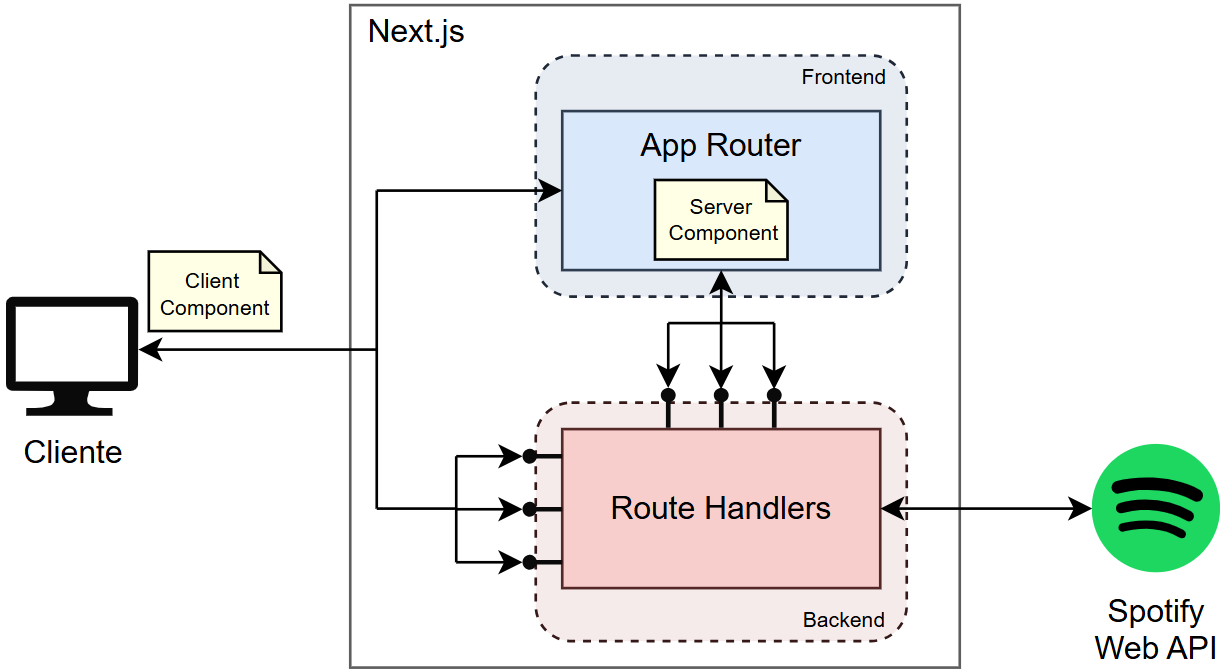
\includegraphics[width=0.85\textwidth]{figures/arquitectura_sistema.png}
    \caption{Diagrama de la arquitectura del sistema haciendo uso de \textit{Next.js}.}
    \label{fig:arquitectura_sistema}
\end{figure}

\subsection{Rutas del Frontend}

Usando el \textit{App Router}, las rutas del frontend se organizan en la carpeta \texttt{app/}, donde cada subcarpeta representa una ruta específica en la web. Dentro de cada carpeta se pueden encontrar archivos específicos que siguen una convención de nombres, y que definen su función. Las más importantes son:

\begin{itemize}
    \item \texttt{layout.tsx}: Define el diseño compartido de los componentes que se encuentran anidados en las subcarpetas interiores.
    \item \texttt{page.tsx}: Contiene el contenido principal de una ruta específica. Representa la página renderizada cuando el usuario accede a esa ruta. \textbf{Para que una página sea accesible, debe existir un archivo \texttt{page.tsx} en la carpeta correspondiente}.
    \item \texttt{loading.tsx}: Muestra un indicador de carga mientras se obtienen datos o se renderizan componentes en una página.
    \item \texttt{error.tsx}: Gestiona errores específicos de una página, mostrando mensajes o interfaces para el usuario en caso de fallos.
\end{itemize}

En el caso de este proyecto, la jerarquía de carpetas que genera las páginas routeables de la web es la siguiente:

\begin{verbatim}
    app/
    ├── home/
    │   └── page.tsx (Ruta: /home)
    ├── stats/
    │   └── page.tsx (Ruta: /stats)
    └── page.tsx (Ruta: /)
\end{verbatim}

La ruta \texttt{/} (raíz) es la página principal, en donde el usuario puede iniciar sesión. Las rutas \texttt{/home} y \texttt{/stats} representan las páginas de estadísticas básicas y estadísticas avanzadas, respectivamente. En cada caso, el archivo \texttt{page.tsx} define el contenido principal de la página y es posible añadir otros archivos como \texttt{layout.tsx}, \texttt{loading.tsx} o \texttt{error.tsx} para mejorar la experiencia del usuario.

\subsection{Endpoints del Backend}

En el caso de la creación de endpoints mediante los \textit{Route Handlers}, la estructura de carpetas es similar a la de las rutas del frontend, pero con la diferencia de que cada subcarpeta dentro de \texttt{app/api/} contiene un archivo \texttt{route.ts} que define el comportamiento del endpoint asociado. \textbf{Para que un endpoint sea accesible, debe existir un archivo \texttt{route.ts} en la carpeta correspondiente}.

La estructura de carpetas para los endpoints de este proyecto es la siguiente:

\newpage

\begin{verbatim}
    app/
    └── api/
        ├── auth/
        │   ├── callback/route.ts
        │   ├── login/route.ts
        │   └── logout/route.ts
        ├── home/
        │   ├── recently-played/route.ts
        │   ├── top-artists/route.ts
        │   ├── top-genres/route.ts
        │   ├── top-tracks/route.ts
        │   └── user-profile/route.ts
        └── stats/
            ├── estaciones-musicales/route.ts
            ├── hall-of-fame/route.ts
            ├── huella-del-dia/route.ts
            ├── indice-de-resonancia/route.ts
            ├── la-bitacora/route.ts
            └── tus-decadas/route.ts
\end{verbatim}

Los endpoints en \texttt{/api/auth/} gestionan el incio de sesión del usuario, mientras que los de \texttt{/api/home/} y \texttt{/api/stats/} se encargan de obtener y procesar los datos necesarios para las estadísiticas. El contenido del fichero \texttt{route.ts} sigue una convención concreta que \textit{Next.js} reconoce y utiliza para gestionar las peticiones, la cual se explicará con más detalle en el capítulo de \nameref{ch:implementacion}.

\section{Diagrama de Componentes de React} \label{sec:diagrama_componentes_react}

Los componentes en \textit{React} son las piezas fundamentales para construir interfaces de usuario. Cada componente puede ser reutilizable, contener su propio estado y lógica, y ser combinado con otros para formar estructuras más complejas. Para describir estas interfaces de manera declarativa, \textit{React} utiliza \textbf{JSX} (JavaScript XML), una extensión de sintaxis de JavaScript, que permite escribir el código de los componentes con una sintaxis similar a \textit{HTML}. Aunque no sea obligatorio, su uso es ampliamente adoptado en proyectos \textit{React}.

Las interfaces se suelen diseñar en forma de jerarquías de componentes, en las que los componentes ``padre'' organizan y controlan el comportamiento y la presentación de los componentes ``hijo''. Esta organización jerárquica facilita el mantenimiento y la escalabilidad del código, ya que cada componente tiene una responsabilidad definida. En este proyecto, se ha creado una jerarquía de componentes (diagrama \ref{fig:componentes_react}) que refleja las diferentes funcionalidades de la aplicación. A la hora de construir la web, \textit{Next.js} y \textit{React} se encargan de anidar los componentes necesarios y renderizarlos, o enviarlos al cliente, según sea necesario.

\begin{figure}[H]
    \centering
    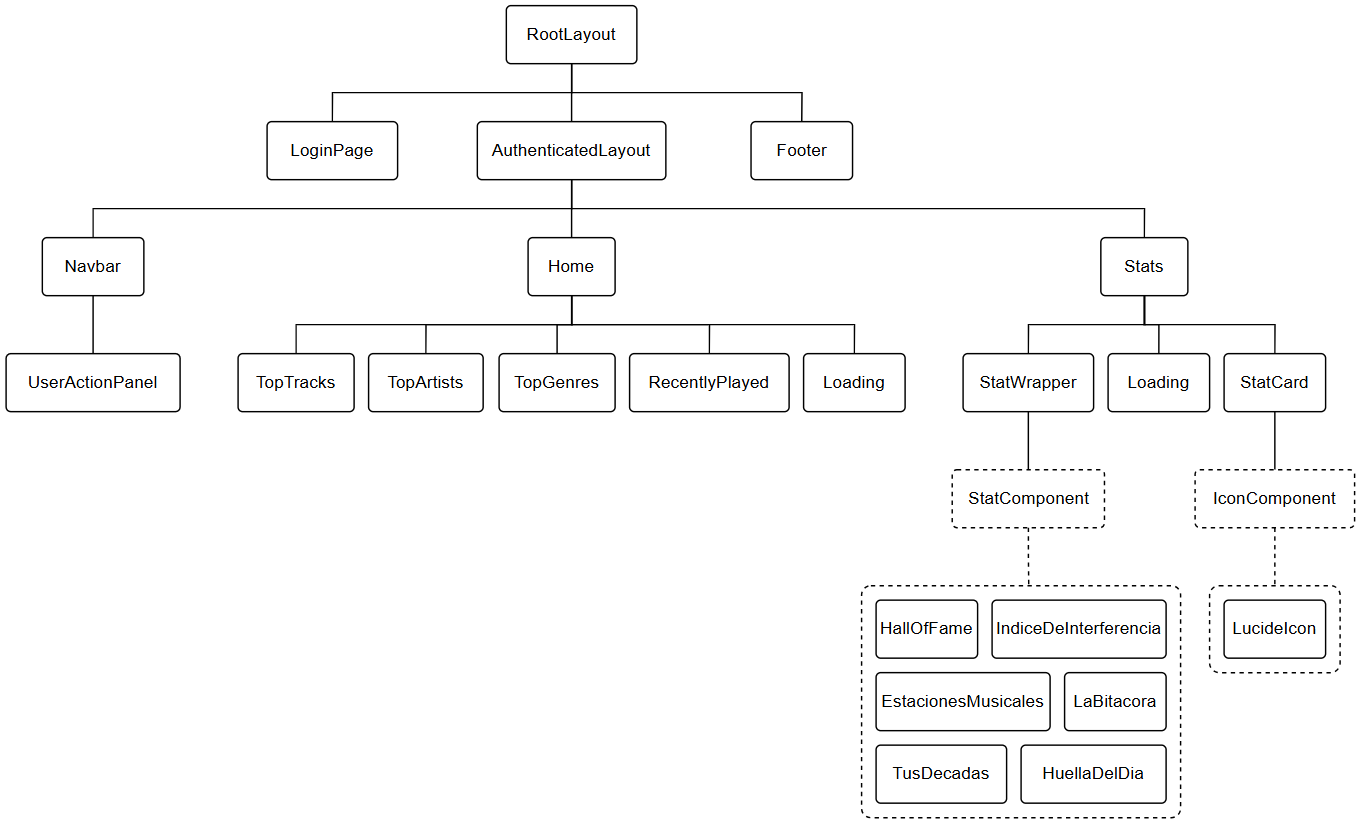
\includegraphics[width=\textwidth]{figures/componentes_react.png}
    \caption{Diagrama de la jerarquía de componentes de React creados en el proyecto.}
    \label{fig:componentes_react}
\end{figure}

Como se muestra en el diagrama, se pueden diferenciar tres tipos diferentes de compontentes, según sus características. \textit{React} define dos principales clases: los \textbf{Client Components} y, los ya mecionados, \textbf{Server Componens}. \textit{Next.js} hace uso concreto de esta diferenciación para optimizar las páginas. Como su nombre indica, los \textit{client components} son componentes de \textit{React} que se ejecutan en el navagador del cliente. Para ello, es necesario enviar toda la lógica junto con el HTML y los estilos, haciendo que este tipo de componentes sean más pesados y requieran más computación por parte de la máquina del usuario. Como respuesta, se introdujeron los \textit{server components}, para que los componentes que no contuviesen funcionalidades de interacción complejas pudieran ser renderizados en el servidor, enviando solamente el HTML y los estilos necesarios al cliente. Con esto se reduce considerablemente la carga del navegador y mejora la rapidez de la web.

El tercer tipo de componente, los \textbf{Loading Components}, no son una clasificación oficial, si no que se ha querido hacer una diferenciación con respecto a los componentes ``comunes''. No añaden funcionalidad ni información concreta a la página, solamente se usan como sustitutos temporales mientras se cargan los componentes finales. Son especialmente útiles para usarlos junto con los \textit{server components}, ya que estos pueden tardar en ser enviados al cliente por el proceso de renderizado (y carga de datos) en el servidor. Hasta entonces, \textit{Next.js} recurre a mostrar el \textit{loading component} para dar un feedback al usuario (figura \ref{alg:suspense_fallback}). Además, estos componentes pueden modelarse de tal forma que representen el ``esqueleto'' del estilo del componente final. Todo esto permite que el proceso de carga se sienta más rápido e informativo, mejorando la experiencia del usuario.

% Ajustar espacios antes de este entorno
\setlength{\intextsep}{15pt} % Espacio superior
\setlength{\abovecaptionskip}{0pt} % Espacio antes del título
\setlength{\belowcaptionskip}{0pt} % Espacio entre título y texto posterior

\begin{ifalgorithm}[H]
    \begin{lstlisting}
    <Suspense fallback={<UserProfileSkeleton />}>
        <UserProfile />
    </Suspense>
    \end{lstlisting}
    \caption{Entorno \texttt{Suspense} para mostrar un fallback mientras se carga el componente \texttt{UserProfile}.}
    \label{alg:suspense_fallback}
\end{ifalgorithm}

Por último, hay algunos componentes que se han definido para realizar cargas dinámicas. El contenido no será enviado hasta que el usuario realice alguna acción que dispare una petición a \textit{Next.js}, sustituyendo en el lugar indicado uno de los componentes preestablecidos. En este proyecto, se han definido dos componentes que se comportan así:

\begin{itemize}
    \item \textbf{Dialog}: Se utiliza para cargar en una ventana modal una de las seis estadísticas disponibles, cada una siendo un componente autocontenido. Dependiendo de la selección del usuario, se cargará uno de estos subcomponentes en el lugar correspondiente. También se puede inferir que solo se podrá mostrar una estadística a la vez.
    \item \textbf{IconComponent}: Está asociado con los iconos representativos de cada estadística, que se muestran en las tarjetas (\texttt{StatCard}) y que el usuario puede clicar para ver. Utiliza el paquete \texttt{LucideIcon} para cargar diferentes iconos, ya que, en este paquete, cada icono es representado como un componente de \textit{React}.
\end{itemize}

Utilizando de manera consciente estas herramientas del framework, se reduce la cantidad de código a enviar al cliente. En el caso de este proyecto, se ha procurado usar, en la medida de lo posible, los \textit{server components}; solo recurriendo al uso de los \textit{client components} en casos necesarios, ya sea por la gestión de estados para interactividad avanzada o llamadas a endpoits de datos.

\section{Interfaz de Usuario}

La interfaz de usuario es uno de los aspectos más flexibles dentro del desarrollo de software, ya que permite una gran libertad creativa y de implementación. En este proyecto, se plantearon varias opciones: utilizar una base de diseño preexistente, como guías visuales o sistemas de diseño consolidados, o desarrollar una interfaz completamente personalizada. Debido a que este trabajo pertenece al ámbito de la informática y no del diseño gráfico, muchas decisiones se orientaron hacia la practicidad, priorizando herramientas y enfoques que permiten simplificar el desarrollo, sin sacrificar la experiencia de usuario. A continuación, se describen las decisiones tomadas al respecto.

\subsection{Principios de Diseño}

Como \textit{Spotify} es una plataforma ampliamente conocida y tiene una identidad visual muy reconocible, se decidió inspirar la interfaz en su diseño. La plataforma propociona una guía para los desarrolladores que incluye recomendaciones muy útiles \cite{spotifyDesign2025}. De entre ellas, se han seleccionado aquellos elementos que resultan relevantes para el uso y alcance de esta aplicación, que se sintetizan en los siguientes puntos:

\subsubsection*{Colores}

El principal identificador visual de \textit{Spotify} es su color verde, llamado \textbf{Spotify Green}. Este color es el que se ha utilizado como el color primario para la página web. Además, se han incorporado el blanco y negro oficiales y también algunos colores complementarios, como el zul y el rojo, para aportar variedad en las situaciones en las que se necesite.

\begin{figure}[H]
    \centering
    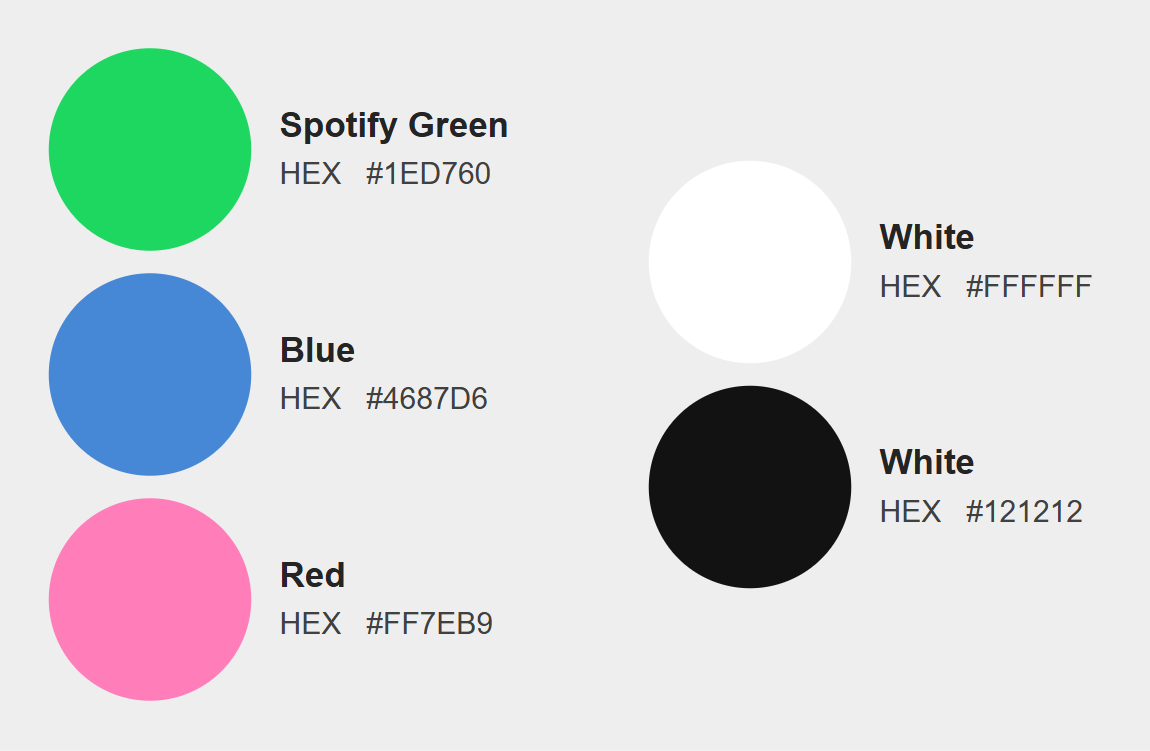
\includegraphics[width=0.5\textwidth]{figures/colores_usados.png}
    \caption{Colores seleccionados para la paleta de colores de la aplicación.}
    \label{fig:colores_usados}
\end{figure}

Estas combinaciones respetan las recomendaciones de la plataforma, que desaconseja el uso de colores sobresaturados, y también se ha ajustado claridad de los colores en ciertas ocasiones para mejorar el contraste en la lectura de texto.

\subsubsection*{Tipografía}

Aunque \textit{Spotify} no proporciona acceso público a su tipografía ofical, sugieren usar fuentes sans-serif como \textit{Helvetica} o \textit{Arial}. En el caso de este proyecto, se ha optado por hacer uso de la tipografía \textbf{Inter} (figura \ref{fig:inter_fuente}), ya que se asemeja más a la original que las recomendadas. Podemos encontrarla en \textit{Google Fonts}, pero \textit{Next.js} nos evita la necesidad de tener que descargarla, ya que está incluida de forma predeterminada en el framework.

\begin{figure}[H]
    \centering
    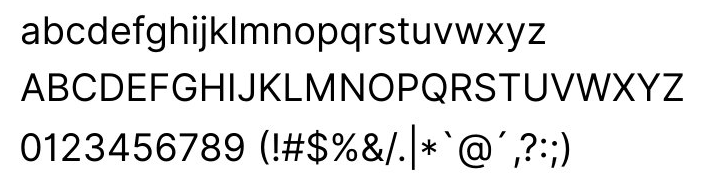
\includegraphics[width=0.6\textwidth]{figures/inter_fuente.png}
    \caption{Muestra de caracteres de la tipografía \textit{Inter}.}
    \label{fig:inter_fuente}
\end{figure}

\subsection{Tailwind CSS}

Para el estilizado de los elementos de la interfaz se ha utilizado \textit{Tailwind CSS}, una librería de utilidades que permite desarrollar estilos de manera rápida y eficiente. En vez de crear un estilo agrupado que se asocie a cada elemento, el enfoque de \textit{Tailwind} se basa en agregar pequeñas clases utilitarias predefinidas a cada elemento mediante el atributo \texttt{className} en JSX (figura \ref{alg:ejemplo_tailwind}), aplicandole así el resultado de la combinación de todos esos estilos.

% Ajustar espacios antes de este entorno
\setlength{\intextsep}{15pt} % Espacio superior
\setlength{\abovecaptionskip}{0pt} % Espacio antes del título
\setlength{\belowcaptionskip}{0pt} % Espacio entre título y texto posterior

\begin{ifalgorithm}[H]
    \begin{lstlisting}
    <main className="flex flex-col items-center justify-center">
    <h1 className="text-2xl font-bold mb-4">Bienvenido</h1>
    <a href="/api/auth/login"
        className="px-4 py-2 bg-green-500 text-white rounded">
    Sign In </a>
    </main>
    \end{lstlisting}
    \caption{Ejemplo de aplicación de estilos a un componente JSX usando \textit{Tailwind CSS}.}
    \label{alg:ejemplo_tailwind}
\end{ifalgorithm}

De esta manera se evita la necesidad de definir manualmente grandes cantidades de estilos en archivos CSS. Además de los estilos estéticos, \textit{Tailwind} aporta muchas clases relacionadas con la adaptavilidad de los componentes a diferentes dispositivos, para generar interfaces \textit{responsive} con facilidad.

Otra razón por la que se ha decidido utilizar este sistema, es su integración con \textit{React} y \textit{Next.js}. Es un stack de tecnologías frontend muy popular, por lo que existe mucha documentación al respecto y se garantiza una gran compatibilidad. Además, \textit{Tailwind} es muy flexible y permite personalizar los estilos de manera sencilla para ajustarlos a cualquier tipo de proyecto.

\subsection{Páginas y Componentes Principales}

Para finalizar con la cacterización de la interfaz de usuario, se presentarán los componentes de la web, la distribución de los elementos dentro de ella y las decisiones tomadas al respecto. Dado el enfoque más técnico de este documento, solo se han incluido las figuras de los componentes principales. Los detalles específicos de cada estadística y elementos secundarios de la interfaz se han trasladado al \hyperref[ch:anexoA]{Anexo A}.

La primera página presentada al usuario es la página de \textbf{inicio de sesión} (figura \ref{fig:login}), que se encuentra en la ruta raíz. Solo se presenta una interacción posible, que es con el botón de \textit{Log In}. Además de la parte puramente funcional, esta pantalla inicial permite una introducción visual al estilo de la web, centrado en los colores ya presentados y la decisión de usar un fondo negro, al igual que la aplicación nativa de \textit{Spotify}.

\begin{figure}[H]
    \centering
    
\includegraphics[width=0.75\textwidth]{figures/capturas_ui/login.png}
    \caption{Página de inicio de sesión del proyecto.}
    \label{fig:login}
\end{figure}

Una vez dentro, la navegación entre las diferentes secciones se realiza a través de una \textbf{barra de navegación} (figura \ref{fig:navbar}), accesible en todo momento. En esta barra se incluyen el logo y nombre de la aplicación, los botones de navegación principales y el perfil del usuario. Desde este último, el usuario puede cerrar sesión en cualquier momento mediante la opción de \textit{Log Out}. Este elemento fijo en la interfaz facilita la orientación dentro de la aplicación y permite un acceso rápido a las secciones esenciales.

\begin{figure}[H]
    \centering
    
\includegraphics[width=0.9\textwidth]{figures/capturas_ui/navbar.png}
    \caption{Barra de navegación fijada en la parte superior de la web.}
    \label{fig:navbar}
\end{figure}

La primera sección tras el inicio de sesión es el \textbf{Home} (\ref{fig:home}), donde se presentan las estadísticas básicas del usuario. Para organizar la información, se ha optado por un diseño basado en módulos, que encapsulan cada una de las estadísticas. Demás del los datos del perfil del usuario, se muestran los tres tops (\textit{Top Tracks}, \textit{Top artists} y  \textit{Top Genres}). Justo debajo, manteniendo una separación, se encuentra la sección de \textit{Recently Played}, que se puede ver al desplazar la ventana.

\begin{figure}[H]
    \centering
    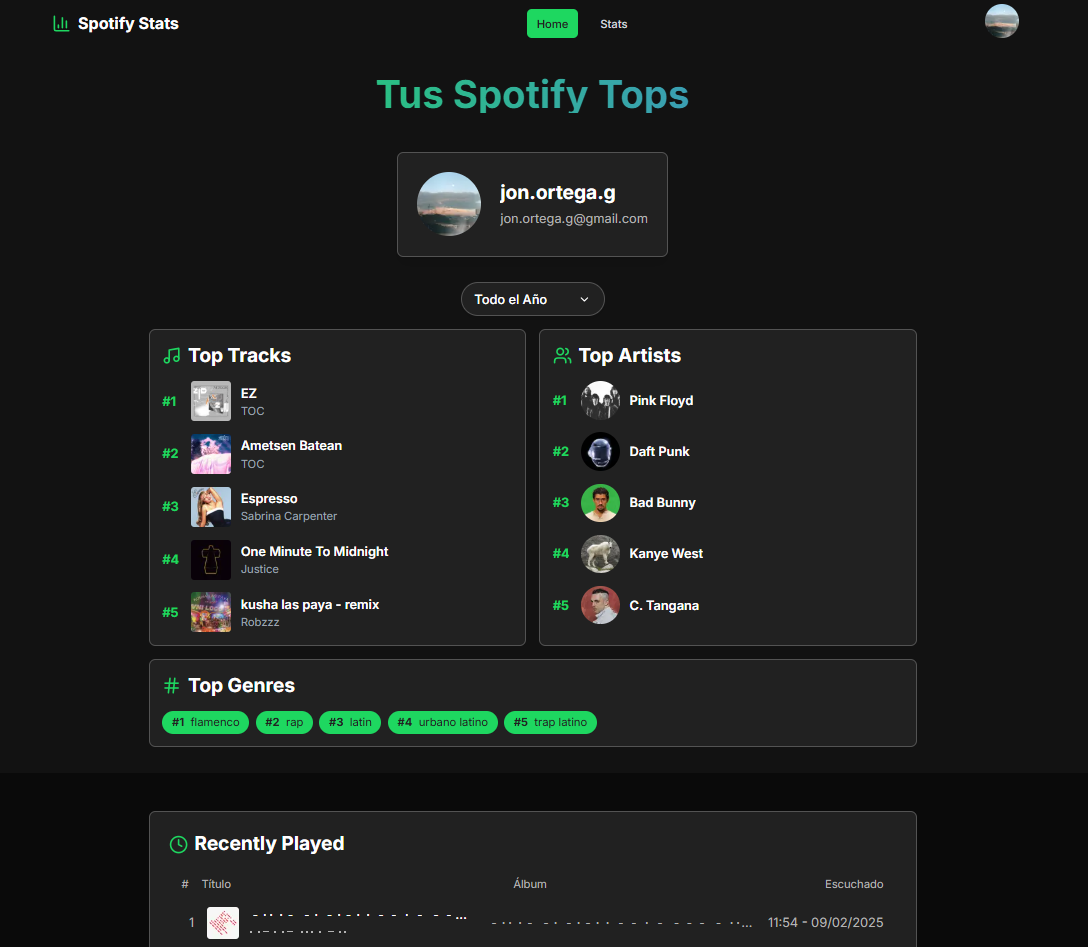
\includegraphics[width=0.65\textwidth]{figures/capturas_ui/home.png}
    \caption{Página de \textit{Home} con las estadísticas básicas.}
    \label{fig:home}
\end{figure}

La segunda gran sección es la de \textbf{Stats} (figura \ref{fig:stats}), donde se han implementado las estadísticas avanzadas. Al igual que en el \textit{Home}, se mantiene el diseño modular basado en tarjetas, pero en este caso con una disposición más flexible para generar una presentación más interesante. Al hacer clic sobre cualquiera de ellas, se abre una \textbf{ventana modal} (figura \ref{fig:modal}) sobre la página, en la que se carga y renderiza la estadística seleccionada. Oscureciendo y difuminando el fondo, se da una sensación de profundidad y crea una separación para foco en la estadísitica. El usuario puede cerrar la ventana modal en cualquier momento haciendo clic fuera de ella o mediante el botón de cierre.

\begin{figure}[H]
    \centering
    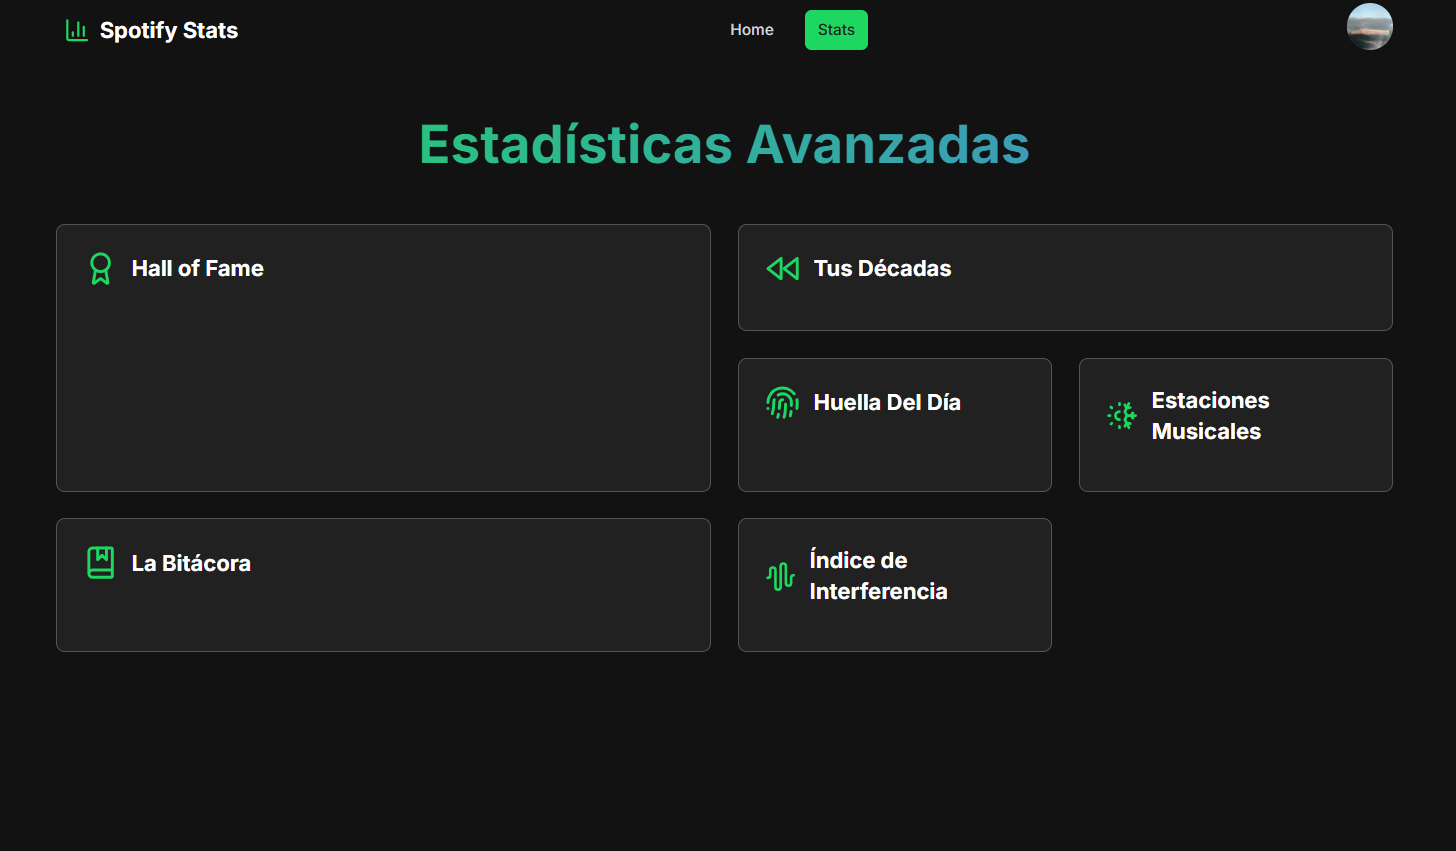
\includegraphics[width=0.65\textwidth]{figures/capturas_ui/stats.png}
    \caption{Página de \textit{Stats} con las tarjetas de estadísticas avanzadas.}
    \label{fig:stats}
\end{figure}

\begin{figure}[H]
    \centering
    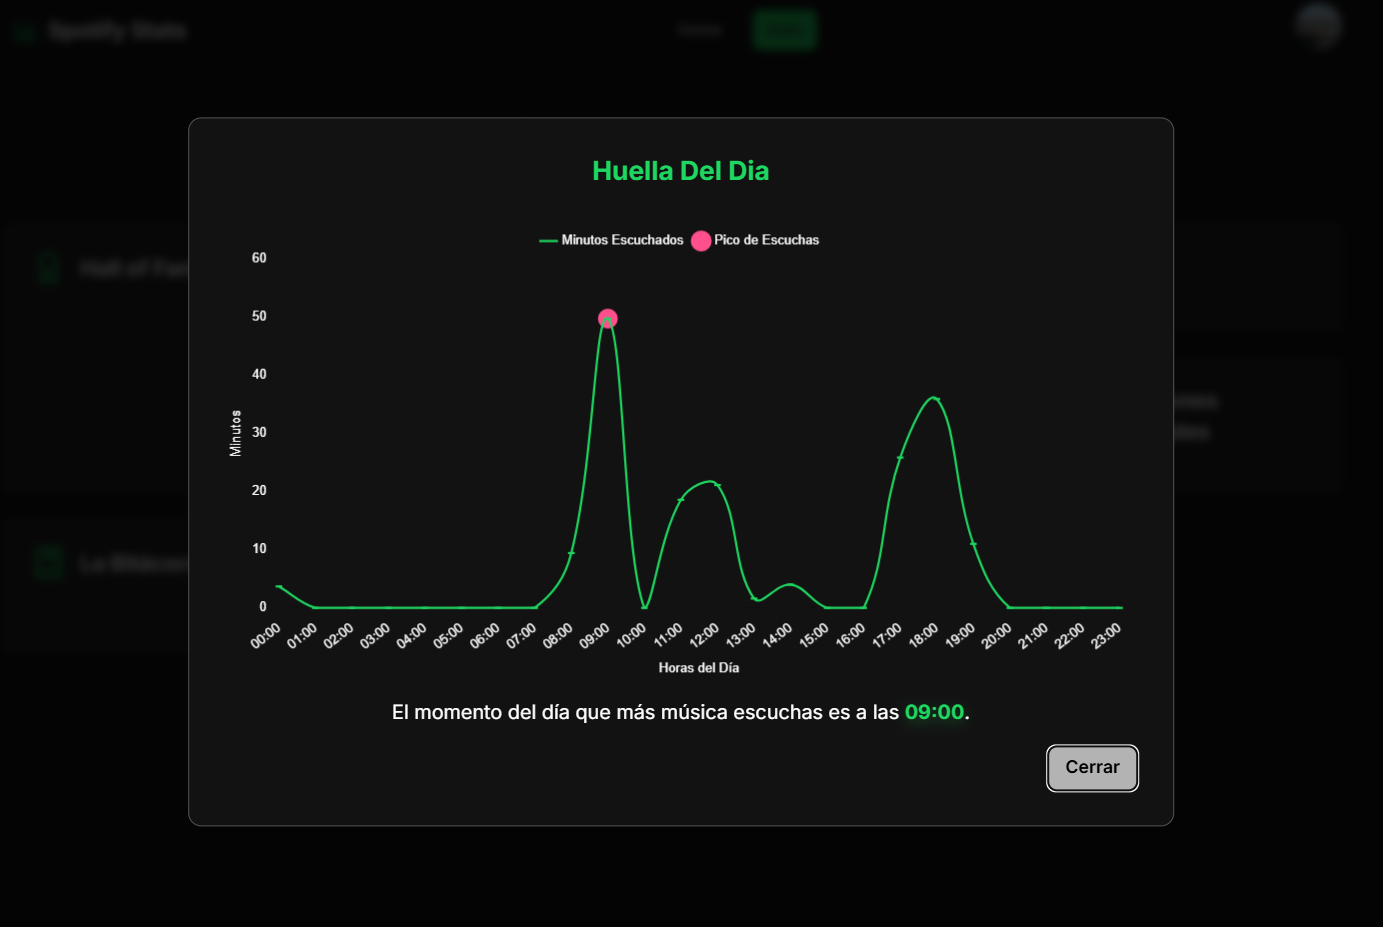
\includegraphics[width=0.65\textwidth]{figures/capturas_ui/modal.png}
    \caption{Ventana modal que contendrá la estadística a mostrar (en este ejemplo, \textit{Huella Del Día}).}
    \label{fig:modal}
\end{figure}

Finalmente, en la parte inferior de la web se encuentra el \textbf{footer} (\ref{fig:footer}), un elemento presente en todas las páginas, incluyendo la pantalla de inicio de sesión. Su función principal es proporcionar un botón para el acceso a la política de privacidad, requisito de los términos de \textit{Spotify} para el uso de su API. Al igual que en las estadísticas, la información se muestra en una ventana modal, evitando la necesidad de cargar una nueva página y manteniendo la coherencia en la interacción del usuario con la aplicación.

\begin{figure}[H]
    \centering
    
\includegraphics[width=0.85\textwidth]{figures/capturas_ui/footer.png}
    \caption{\textit{Footer} anclado al pie de todas las páginas de la web.}
    \label{fig:footer}
\end{figure}

Aunque las figuras incluidas en el documento hayan sido capturadas en una pantalla de escritorio, todos los elementos dentro de los componentes han sido implementados con un diseño \textit{responsive} en mente, asegurando una visualización clara tanto en pantallas grandes como en dispositivos móviles con pantallas más reducidas.

\newpage

\section{Diagramas de Secuencia}

En esta sección se presentan los diagramas de secuencia más importantes. Se han seleccionado aquellos que presentan una complejidad particular o requieren una explicación más detallada para su correcta interpretación. El resto de los diagramas correspondientes a los casos de uso estarán disponibles en el \hyperref[ch:anexoB]{Anexo B}.

\subsection*{Iniciar Sesión}

Aunque la acción para el usuario sea simple, este caso de uso requiere varios pasos y llamadas a la API de \textit{Spotify} por parte de la lógica de la aplicación. La complejidad viene principalmente viene de la gestión de los errores, ya que, durante este proceso, existen dos puntos en los que el usuario puede rechazar (o ser rechazado) el inicio de sesión. Esos dos casos son: si el usurio introduce las credenciales incorrectas en la autenticación o si el usuario decide no dar la autorización necesaria a la aplicación para trabajar con sus datos. En el diagrama \ref{fig:ds_iniciar_sesion} se caracterizan todas estas posibilidades con los marcos de interacción alternativas.

\begin{figure}[H]
    \centering
    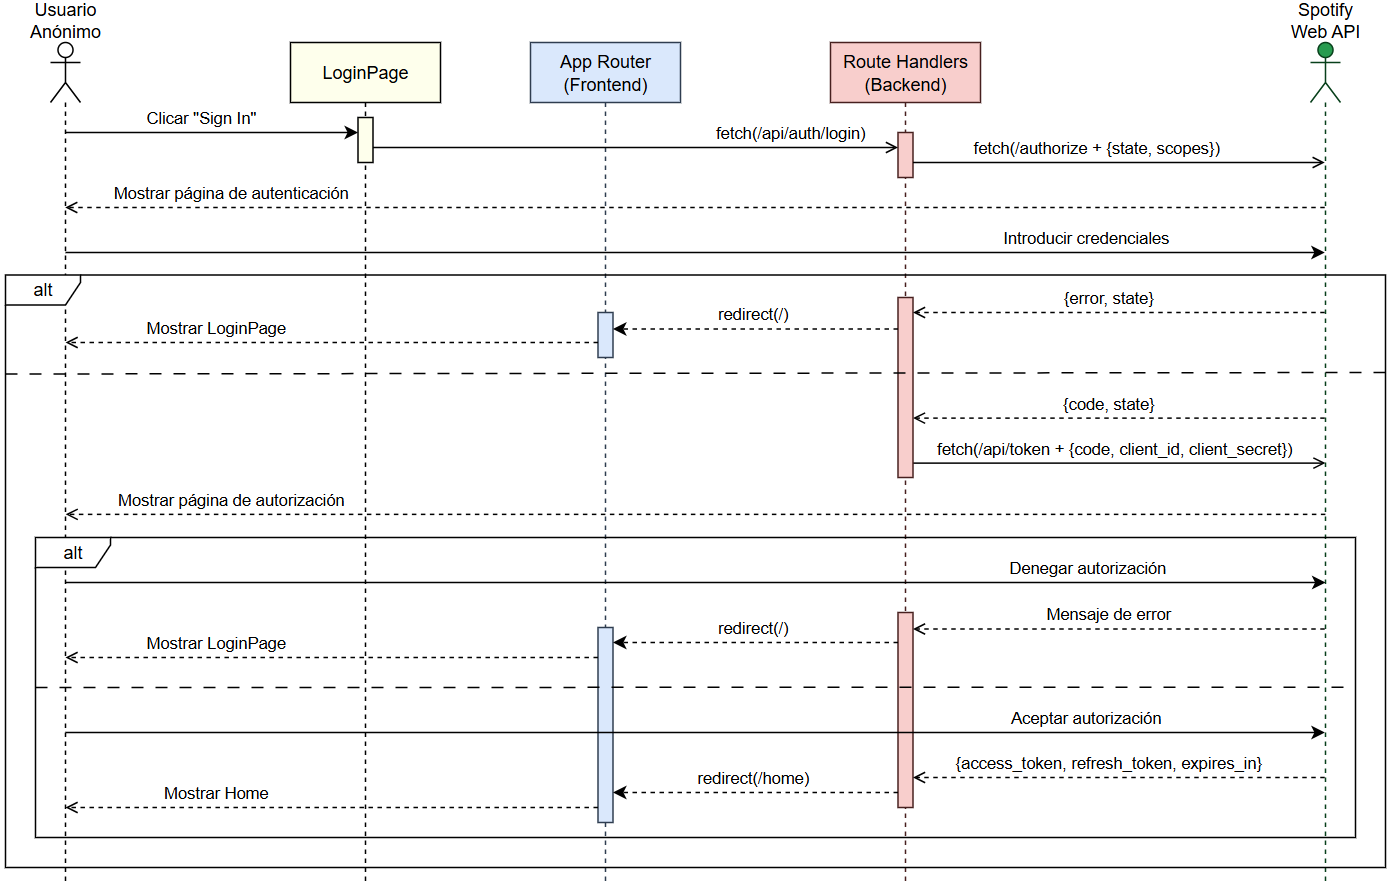
\includegraphics[width=\textwidth]{figures/diagramas_secuencia/ds_iniciar_sesion.png}
    \caption{Diagrama de secuencia: Iniciar Sesión.}
    \label{fig:ds_iniciar_sesion}
\end{figure}

\subsection*{Acceder a Home}

En este este caso de uso, la aplicación carga la página de \textit{Home} junto con todos los componentes de las estadísticas básicas. En el diagrama \ref{fig:ds_acceder_home} se muestra un marco que representa un proceso paralelo. Se ha querido remarcar esta característica de la carga, ya que todos los componentes se renderizan de manera asíncrona, gracias a la funcionalidad del entorno \textsl{Suspense} de \textit{Next.js} mencionado en la sección \nameref{sec:diagrama_componentes_react}.

\begin{figure}[H]
    \centering
    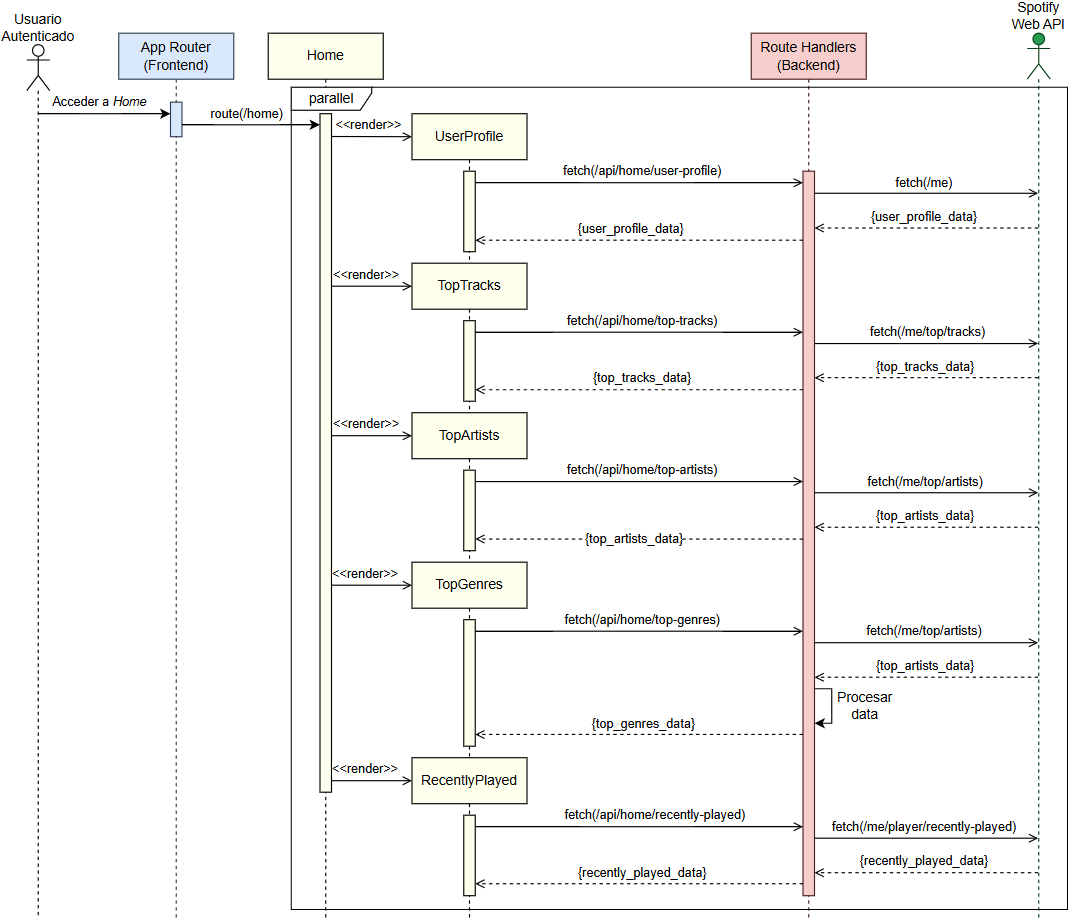
\includegraphics[width=\textwidth]{figures/diagramas_secuencia/ds_acceder_home.png}
    \caption{Diagrama de secuencia: Acceder a \textit{Home}.}
    \label{fig:ds_acceder_home}
\end{figure}

\subsection*{Acceder a Stats}

Al acceder a la página de \textit{Stats}, se renderizan varias instancias del mismo componente \textsl{StatCard}, una para cada estadística. Luego, cuando el usuario selecciona una de ellas, el componente envía el \texttt{statId} de la estadística correspondiente al componente \texttt{StatWrapper}. Por último, el \texttt{StatWrapper} renderizará el componente asociado al indentificador de manera dinámica, cuyos diagramas de secuencia se han definido de manera independiente. El acceso a \textit{Stats} se ha caracterizado en el siguiente diagrama \ref{fig:ds_acceder_stats}:

\begin{figure}[H]
    \centering
    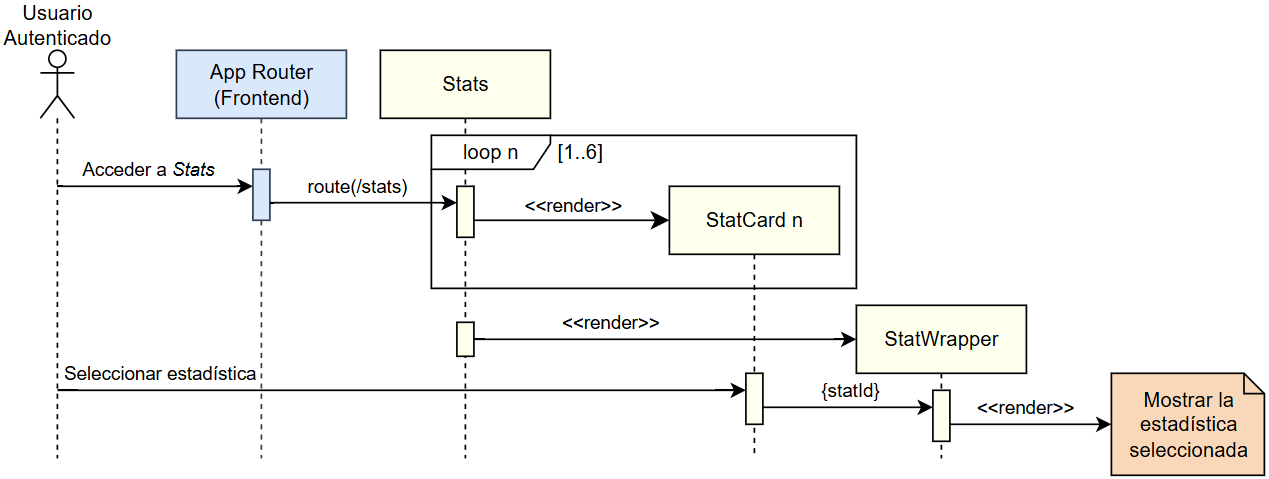
\includegraphics[width=0.9\textwidth]{figures/diagramas_secuencia/ds_acceder_stats.png}
    \caption{Diagrama de secuencia: Acceder a \textit{Stats}.}
    \label{fig:ds_acceder_stats}
\end{figure}

\subsection*{Ver Hall Of Fame}

El renderizado y la carga de la estadística \textit{Hall Of Fame} se realiza de manera estándar, pero ofrece una funcionalidad añadida, identificado con el caso de uso extendido \textbf{Crear Playlist} (diagrama \ref{fig:ds_ver_hall_of_fame}). Al clicar sobre el botón, se realizan varias interacciónes en cadena con la API de \textit{Spotify} para crear la playlist, añadir canciones y establecer una nueva portada.

\begin{figure}[H]
    \centering
    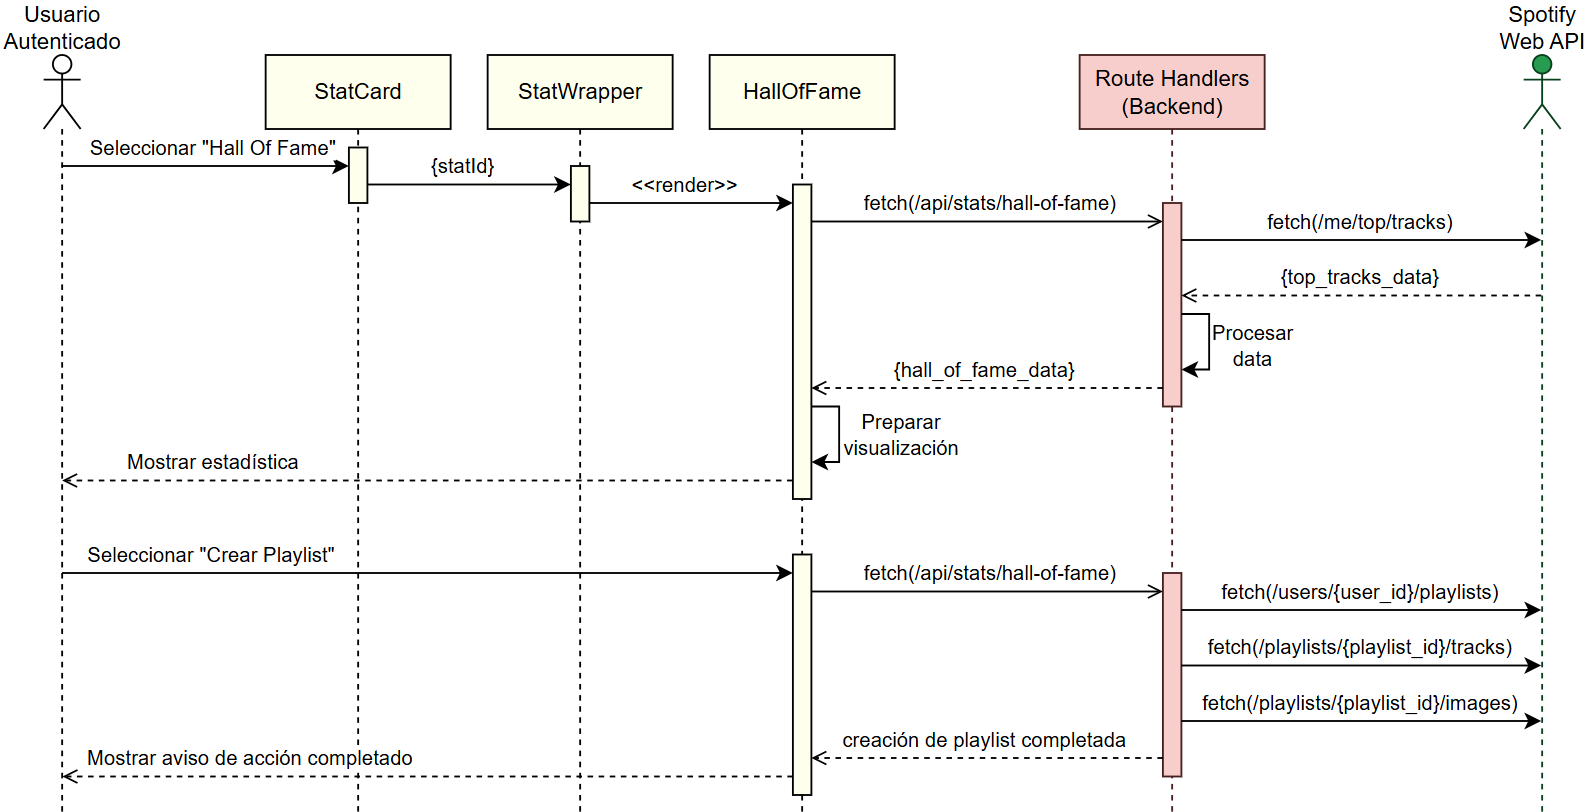
\includegraphics[width=\textwidth]{figures/diagramas_secuencia/ds_ver_hall_of_fame.png}
    \caption{Diagrama de secuencia: Ver Hall Of Fame.}
    \label{fig:ds_ver_hall_of_fame}
\end{figure}

\subsection*{Ver La Bitácora}

En el caso de esta estadística, se permite al usuario navegar entre los distintos niveles temporales de datos. Para evitar consumir constantemente la API de \textit{Spotify}, los datos se cargan en un caché temporal en el servidor. De esta manera, cuando el usuario solicite los datos, se enviarán con menos latencia y se evita la sobrecarga de llamadas a \textit{Spotify}. En el diagrama \ref{fig:ds_ver_la_bitacora} se muestra esa interacción en el marco de bucle.

\begin{figure}[H]
    \centering
    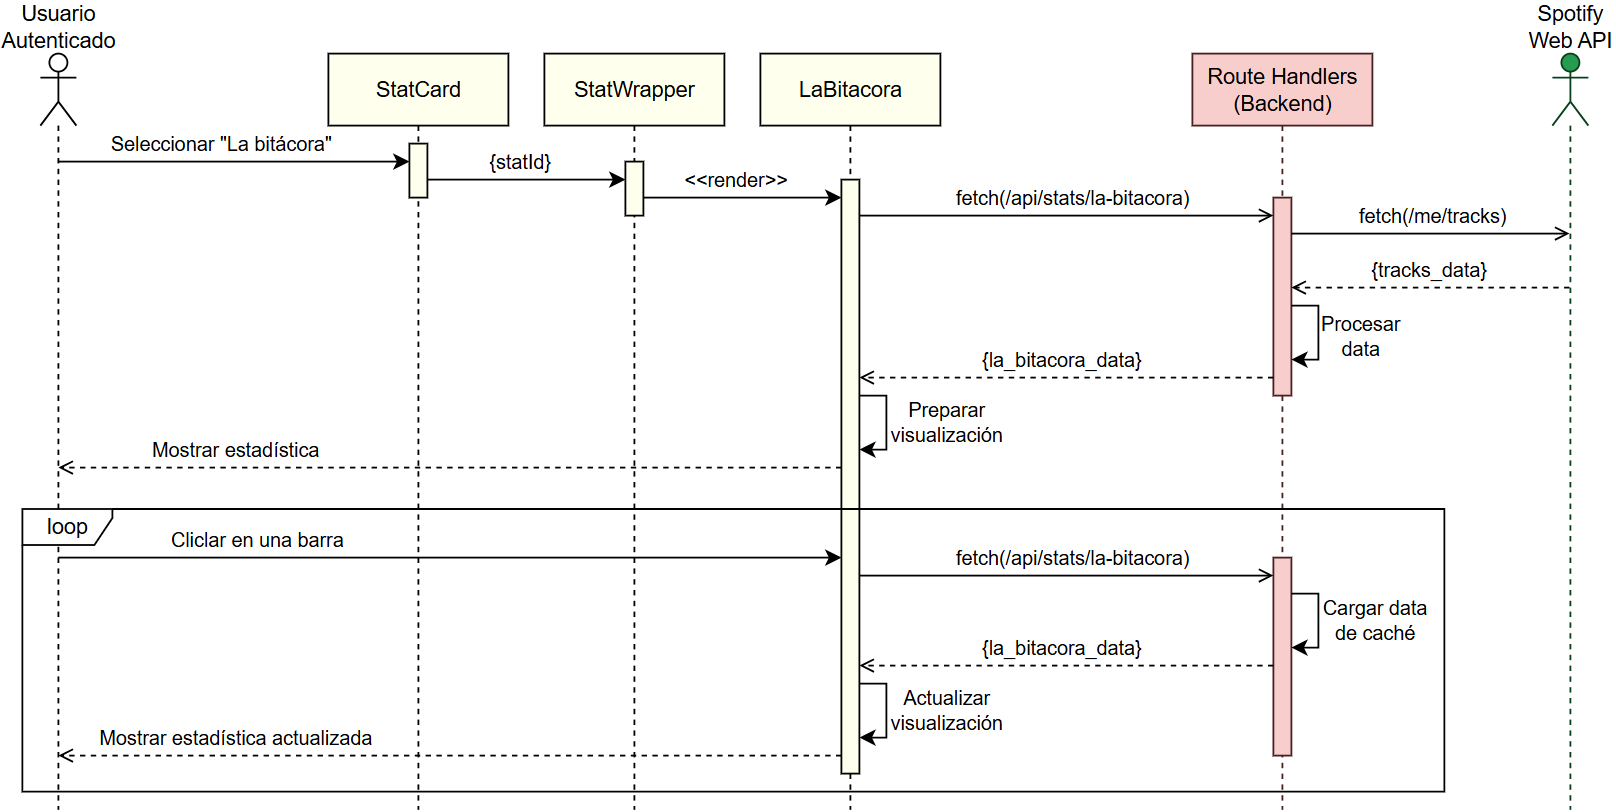
\includegraphics[width=\textwidth]{figures/diagramas_secuencia/ds_ver_la_bitacora.png}
    \caption{Diagrama de secuencia: Ver La Bitácora.}
    \label{fig:ds_ver_la_bitacora}
\end{figure}

\section{Diseño de la Seguridad} \label{sec:diseno_seguridad}

Como esta aplicación maneja información privada de los usuarios, un aspecto crítico en el diseño y desarrollo de la misma es la seguridad. En esta sección se describen las medidas implementadas para proteger los datos de posibles ataques comunes y reducir las vulnerabilidades del sistema.

\subsection{Gestión de Credenciales}

La mala gestión de credenciales es un punto de vulnerabilidad común en aplicaciones web. En el caso del proyecto, se manejan varias credenciales sensibles, especialmente durante el flujo de inicio de sesión. A continuación se detallan las medidas aplicadas a cada una.

\subsubsection*{Client ID y Client Secret}

En la creación de una aplicación que hace uso de la API de \textit{Spotify}, se obtiene un \textbf{client\_id} y un \textbf{client\_secret} que son necesarios para la autenticación con la API. Estas credenciales pertenecen al desarrollador y deben ser protegidas adecuadamente para evitar su exposición a terceros no autorizados. Se almacenan exclusivamente en el servidor, en un archivo de variables de entorno (\texttt{.env.local}), que no se incluye en el control de versiones. En el momento del despliegue, estas variables se cargan en el entorno de producción, que han de ser anteriormente indicadas de manera manual a través de un panel de configuración de \textit{Vercel}. Se puede acceder a estas variables en el lógica del servidor mediante el obtejo \texttt{process.env}.

\subsubsection*{Prevención de CSRF y Scopes}

Para prevenir ataques de \textit{Cross-Site Request Forgery} (CSRF), cada solicitud de inicio de sesión incluye un valor de estado (\textbf{state}) generado de forma aleatoria. Este valor es único para cada sesión y se valida al recibir la respuesta del servidor de autenticación. Este mecanismo, recomendado explícitamente en la documentación de \textit{Spotify} \cite{spotifyAuthCodeFlow2025}, garantiza que las solicitudes sean legítimas y originadas únicamente desde el cliente autorizado, evitando que actores maliciosos puedan ejecutar acciones en nombre del usuario.

Por otro lado, durante el paso de la autorización en el proceso de inicio de sesión, se respeta el principio de mínimos privilegios, donde solo se solicitan los permisos necesarios y ninguno más. Los usuarios son informados claramente sobre los \textbf{scopes} solicitados y su propósito antes de otorgar los permisos. De esta manera se consigue reducir el riesgo de exposición innecesaria de datos.

\subsubsection*{Access Token y Refresh Token}

Una vez que el usuario ha iniciado sesión y la aplicación ha obtenido un \textbf{access\_token} y un \textbf{refresh\_token}, estos se almacenan en unas cookies correspondiente. La configuración de estas cookies es muy importante para protegerlas frente a ataques comunes como \textit{Cross-Site Scripting} (XSS) o \textit{Man-In-The-Middle} (MITM). Las siguientes marcas (\textit{flags}) permiten configurar la seguridad necesaria:

\begin{itemize}
    \item \textbf{\texttt{httpOnly}:} Indicando esta opción como ``\texttt{true}'', asegura que las cookies no puedan ser accedidas por código JavaScript en el navegador, protegiéndolas contra ataques de XSS.
    \item \textbf{\texttt{secure}:} Indicando esta opción como ``\texttt{true}'', las cookies solo pueden ser transmitidas a través de conexiones HTTPS, protegiéndolas contra ataques de MITM. Esta opción solo es necesaria en un entorno de producción, es posible desactivarlo durante el desarrollo.
    \item \textbf{\texttt{maxAge}} Estableciendo un tiempo de vida limitado, se garantiza que se las cookies se eliminen automáticamente una vez cumplido el periodo concretado, minimizando el impacto de un posible compromiso.
\end{itemize}

\subsection{Routing y Conexiones Seguras}

Next.js proporciona un sistema de \textbf{middleware} que permite ejecutar procesos antes de que se manejen las solicitudes de las rutas. En este proyecto, se ha implementado un middleware que verifica la validez de las cookies de sesión antes de permitir el acceso a las rutas protegidas. Si no existe una cookie con un access token, el usuario es redirigido a la página de inicio de sesión, grantizando que solo los usuarios autenticados puedan acceder a las estadísticas y los datos personales.

Para la comunicación entre el cliente y la aplicación, al desplegatse en \textit{Vercel}, éste proporciona automáticamente \textbf{conexiones HTTPS} para todas las solicitudes. Esto garantiza la confidencialidad de los datos transmitidos entre el cliente y el servidor, protegiendo contra ataques de intercepción como el MITM.

\subsection{Otras Medidas}

Del mismo modo que se han implementado mecanismos explícitos para prevenir ataques comunes, la seguridad de una aplicación no solo depende de configuraciones específicas, sino también del entorno de desarrollo y de las prácticas adoptadas a lo largo del ciclo de vida del software. La seguridad implícita, aquella que surge como resultado de buenas prácticas y herramientas adecuadas, desempeña un gran papel.

\begin{itemize}
    \item \textbf{Análisis estático del código con ESLint:} Un linter como \textit{ESLint} permite detectar errores, malas prácticas y patrones potencialmente inseguros en el código TypeScript antes de que lleguen a producción. Integrarlo en el flujo de desarrollo facilita la identificación temprana de vulnerabilidades y la posibilidad de corregirlos antes de que se conviertan en problemas de seguridad.

    \item \textbf{Dependencias actualizadas:} La aplicación se construye sobre versiones recientes y estables de \textit{Next.js}, \textit{React} y \textit{Node.js LTS}, lo que permite beneficiarse de mejoras en seguridad y reducir la exposición a vulnerabilidades conocidas; un riesgo muy común derivado del uso de software obsoleto.

    \item \textbf{Ejecución de pruebas:} Realizar pruebas sistemáticas permite identificar fallos inesperados, comportamientos anómalos o configuraciones incorrectas en la aplicación.

    \item \textbf{Prácticas recomendadas:} Seguir las guías oficiales de seguridad, tanto de la API de \textit{Spotify} como de \textit{Next.js}, garantiza que se cumplen los estándares más recientes.
\end{itemize}
